\documentclass[../DC2017114Bouma.tex]{subfiles}
\begin{document}
\graphicspath{{02_Material/img/}}


%% New chapter %%
\cleartooddpage
\chapter{Modeling of Mechanical Systems with Unilateral Constraints and Spatial Friction}
\section{Mechanical system with unilateral constraints and spatial friction dynamics}
\textbf{Define lambdas and other variables}
We define $\xib=\dot{\qb}$, except at jump-times $\tau_i$. $h_n$ is the normal contact distance and $\zetab_{n}$ and $\zetab_{t}$ represent the relative velocities in normal and tangential direction,  respectively. Then, the continuous dynamics of a mechanical system with unilateral constraints and spatial friction are of the form
\begin{align}
&\Mb(\qb)\dot{\xib} + \Hb(\qb,\xib) = \Sb(\qb)\ub + \sum_{i\in\Ic_c}\left(\wb_{n,i}(\qb)\lambda_{n,i} + \Wb_{t,i}(\qb)\lambdab_{t,i} \right), \label{eq:appcont1}\\
&\text{(Contact Law)},\label{eq:appcont2}\\
&\text{(Friction Law)}.\label{eq:appcont3}
\end{align}

When the system activates a unilateral constraint, impulsive dynamics can cause the state of the system to jump. These dynamics are of the form

\begin{align}
&\Mb(\qb)(\xib^+ - \xib^-) = \sum_{i\in\Ic_c}\left( \wb_{n,i}(\qb)\Lambda_{n,i} + \Wb_{t,i}(\qb)\Lambdab_{t,i}\right), \label{eq:appimp1}\\
&\text{(Impulsive Contact Law)},\label{eq:appimp2}\\
&\text{(Impulsive Friction Law)}.\label{eq:appimp3}
\end{align}

These dynamics are impulsive, and happen at one instance in time. The $^-$ superscript indicates the ante-event state and the $^+$ superscript indicates the post-event state. In the following sections three different methods of describing the contact and friction laws are presented. First a complementarity problem formulation of mechanical systems with unilateral constraints is given, from which later a proximal point formulation and a hybrid system formulation are derived.

\section{Complementarity problem formulation}\label{sec:comp}
\subsection{Signourini's contact law and Poisson's impact law}
To describe the normal contact between rigid bodies Signourini's contact law is used. Since the bodies are impenetrable and reaction forces caused by contact can not prevent the bodies from seperating, both the contact distance $h_{n,i}$ and $\lambda_{n,i}$ can not become negative. Two situations are possible

\begin{enumerate}
\item $h_{n,i}=0\ \wedge\ \lambda_{n,i} \geq 0$ (closed-contact)
\item $h_{n,i}>0\ \wedge\ \lambda_{n,i} = 0$ (open-contact)
\end{enumerate}

These situations are illustrated in Figure~\ref{fig:signourinicontact}, where it can be seen that the two situations are orthogonal. This behavior can be summarized in the complementarity condition

\begin{align}
0\leq h_{n,i}\ \bot\ \lambda_{n,i} \geq 0,\label{eq:signourini}
\end{align}

where the symbol $\bot$ is used to express the orthogonality between $h_{n,i}$ and $\lambda_{n,i}$. The complementarity condition in \eqref{eq:signourini} is called Signourini's contact law.
\begin{figure}[h]
\centering
\begin{subfigure}{0.3\textwidth}
\centering
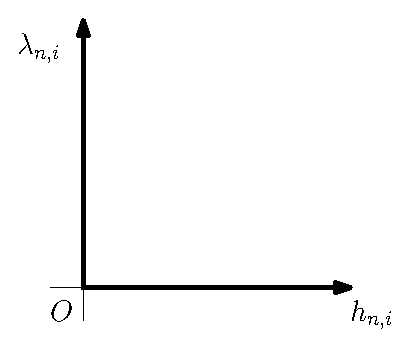
\includegraphics[width=\linewidth]{signourinicontact.eps}
\caption{Signourini's contact law.}\label{fig:signourinicontact}
\end{subfigure}
\qquad
%\begin{subfigure}{0.3\textwidth}
%\centering
%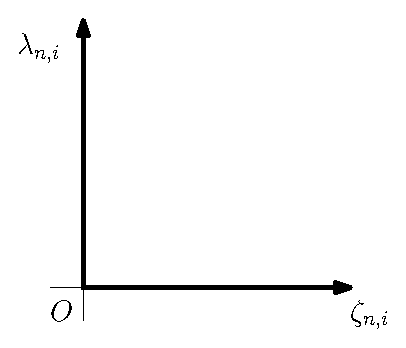
\includegraphics[width=\linewidth]{signouriniforce.eps}
%\caption{Signourini's force law.}\label{fig:signouriniforce}
%\end{subfigure}
%\quad
\begin{subfigure}{0.3\textwidth}
\centering
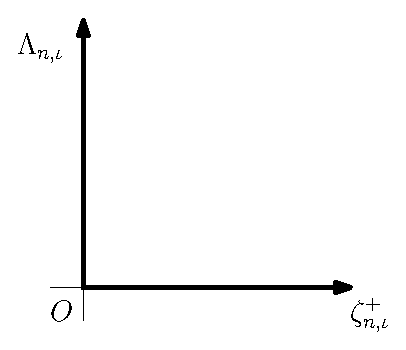
\includegraphics[width=\linewidth]{poissonimpact.eps}
\caption{Poisson's impact law without restitution.}\label{fig:poissonimpact}
\end{subfigure}
\caption{}
\end{figure}

When contact happens at non-zero velocity, impact occurs. Newton's impact law is used to describe this impact. Newton's law of impact is defined as
\begin{align}
\zeta^+_{n,i} = e_{n,i}\zeta^+_{n,i},\text{ when }h_{n,i}=0,\ \dot{h}_{n,i}<0.
\end{align}
In this work the coefficient of restitution $e_{n,i}$ is assumed to be $0$, describing a completely inelastic contact. For closed contact an impact law can be defined that relates the impulsive contact force $\Lambda_{n,i}$ to the post-impact normal velocity $\zeta_{n,i}$. When considering multi-contact systems, when a contact is closed two situations can occur:
\begin{enumerate}
\item $\Lambda_{n,i} > 0\ \wedge\ \zeta^+_{n,i} = 0$ (impact)
\item $\Lambda_{n,i} = 0\ \wedge\ \zeta^+_{n,i} \geq 0$ (no impact)
\end{enumerate}
The second case can occur when a contact point other than $i$ makes impact. The situations described above are illustrated in Figure~\ref{fig:poissonimpact}, where again the orthogonality can be observed. The behavior is written into the complementarity condition

\begin{align}
0\leq \zeta^+_{n,i}\ \bot\ \Lambda_{n,i} \geq 0,\quad  \qquad \forall i\in\Ic_c,\label{eq:poisson}
\end{align}

with $\Ic_c$ the set of closed contacts. The complementarity condition \eqref{eq:poisson} is called Poisson's impact law. Note that the impact law is defined on velocity level, whereas the contact law is defined on position level.
\subsection{Coulomb's friction law}
Coulomb's friction law is often used to describe dry friction in mechanical systems. When considering 3-dimensional environments, Coulomb's friction law is defined as 

\begin{align}
||\lambdab_{t,i}||\ \in\ \left\{ \begin{array}{ll}
||\lambdab_{t,i}||\leq\mu\lambda_{n,i}, &\text{if }||\zetab_{t,i}||=0\\
||\lambdab_{t,i}|| = \mu\lambda_{n,i}, &\text{if }||\zetab_{t,i}||>0
\end{array}\right.,\label{eq:frictionlen}
\end{align}
and since friction is considered isotropic
\begin{align}
\zetab_{t,i} = -\kappa_i\widehat{\lambdab}_{t,i}.\label{eq:frictiondir}
\end{align}
with $\kappa_i>0$ and $\widehat{\xb}$ is the vector length of $\xb$ defined as
\begin{equation}
\widehat{\xb} = \left\lbrace\begin{array}{rr}
\frac{\xb}{||\xb||}, & \text{if } ||\xb|| \neq 0\\
0, & \text{if } ||\xb|| = 0\\
\end{array}\right. .\label{eq:vectorlen}
\end{equation}

\eqref{eq:frictionlen} can be considered as a relation between the magnitude of the tangential velocity $\zetab_{t,i}$ and the reaction friction force $\lambdab_{t,i}$. \eqref{eq:frictiondir} can be considered as a relation between the direction of $\zetab_{t,i}$ and $\lambdab_{t,i}$, namely that $\zetab_{t,i}$ and $\lambdab_{t,i}$ are always in opposite directions. The constant $\kappa_i$ can then be interpreted as the magnitude of the tangential velocity. Coulomb's friction law is illustrated in Figure~\ref{fig:coulombfriction}. In Figure~\ref{fig:coulombort} the same law is illustrated, but now as orthogonal vectors. As noticed earlier, this is convenient for writing the law in a complementarity form.

\begin{figure}[h]
\centering
\begin{subfigure}{0.3\textwidth}
\centering
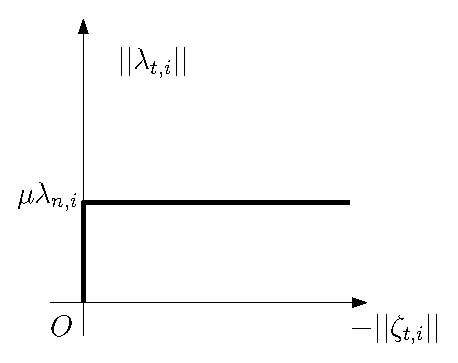
\includegraphics[width=\linewidth]{coulombfriction.eps}\caption{Coulomb's friction law.}\label{fig:coulombfriction}
\end{subfigure}
\qquad
\begin{subfigure}{0.3\textwidth}
\centering
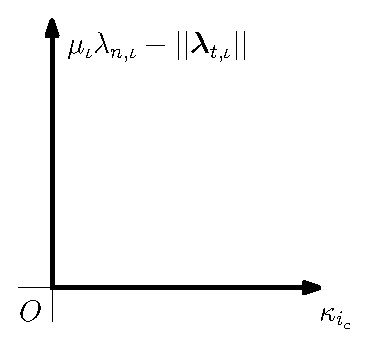
\includegraphics[width=\linewidth]{coulombort.eps}\caption{Coulomb's friction law as orthogonal vectors. $\kappa_i$ is defined as the magnitude of the tangential velocity $\zetab_{t,i}$.}\label{fig:coulombort}
\end{subfigure}
\end{figure}

The complementarity formulation of the Coulomb's law is therefore defined as

\begin{align}
&0\leq \left(\mu\lambda_{n,i} - ||\lambdab_{t,i}||\right)\ \bot\ \kappa_i \geq 0,\label{eq:coulomb1}\\
&\zetab_{t,i} = \kappa_i\widehat{\lambdab}_{t,i}.\label{eq:coulomb2}
\end{align}

For the impulsive behavior of the friction law Newton's impact law is used to define the tangential post-impact velocity as
\begin{align}
\zetab^+_{t,i} = e_{t,i}\zetab^-_{t,i},
\end{align}
where in this work $e_{t,i}=0$ is assumed. Then, similarly to the non-impulsive case, the impulsive Coulomb's friction law can be defined as
\begin{align}
&0 \leq (\mu\Lambda_{n,i} - ||\Lambdab_{t,i}||)\ \bot\ \kappa_i \geq 0. \qquad \forall i\in\Ic_c,\label{eq:coulombimp1}\\
&\zetab_{t,i}^+ = \kappa_i\widehat{\Lambdab}_{t,i},\qquad \forall i\in\Ic_c.\label{eq:coulombimp2}
\end{align}
Note that just as the contact case, the impulsive friction law only holds for closed contacts.
\subsection{System dynamics with contact and friction law}
The flow dynamics are then described by
\begin{align}
&\Mb(\qb)\dot{\xib} + \Hb(\qb,\xib) = \Sb(\qb)\ub + \sum_{i\in\Ic_c}\left(\wb_{n,i}(\qb)\lambda_{n,i} + \Wb_{t,i}(\qb)\lambdab_{t,i} \right), \label{eq:ncpcontact1}\\
&0\leq h_{n,i}\ \bot\ \lambda_{n,i} \geq 0,\label{eq:ncpcontact2}\\
&0\leq \left(\mu\lambda_{n,i} - ||\lambdab_{t,i}||\right)\ \bot\ \kappa_i \geq 0,\label{eq:ncpcontact3}\\
&\zetab_{t,i} = \kappa_i\widehat{\lambdab}_{t,i},\label{eq:ncpcontact4}
\end{align}
with 
\begin{align}
&h_{n,i} = \wb_{n,i}^T(\qb)\qb,\label{eq:h}\\
&\zeta_{n,i}(\qb) = \wb^T_{n,i}(\qb) \xib,  \label{eq:zetan}\\
&\zetab_{t,i}(\qb) = \Wb^T_{t,i}(\qb) \xib. \label{eq:zetab}
\end{align}
The impulsive dynamics that take place when a contact point opens or closes contact are described by
\begin{align}
&\Mb(\qb)(\xib^+ - \xib^-) = \sum_{i\in\Ic_c}\left( \wb_{n,i}(\qb)\Lambda_{n,i} + \Wb_{t,i}(\qb)\Lambdab_{t,i}\right), \label{eq:ncpimpact1}\\
&0\leq \zeta_{n,i}^+\ \bot\ \Lambda_{n,i} \geq 0, \qquad \forall i\in\Ic_c,\label{eq:ncpimpact2}\\
&0 \leq (\mu\Lambda_{n,i} - ||\Lambdab_{t,i}||)\ \bot\ \kappa_i \geq 0. \qquad \forall i\in\Ic_c,\label{eq:ncpimpact3}\\
&\zetab_{t,i}^+ = \kappa_i\widehat{\Lambdab}_{t,i},\qquad \forall i\in\Ic_c,\label{eq:ncpimpact4}
\end{align}
with 
\begin{align}
&\zeta^+_{n,i}(\qb) = \wb^T_{n,i}(\qb) \xib^+,\\
&\zetab^+_{t,i}(\qb) = \Wb^T_{t,i}(\qb) \xib^+.\label{eq:ncpimpactend}
\end{align}

\section{Proximal point formulation}
The contact law and friction law defined in the complementarity condition formulation can be redefined to a proximal point formulation. This makes the system compatible with simulation methods as timestepping \cite[Chapter 10]{Acary2008}. More information on the definition of the proximal point formulation of contact laws and friction laws can be found in \cite[Section 5.3]{Leine2008}.

\subsection{Signourini's contact law and Poisson's impact law}
In Figure~\ref{fig:convex} a convex set $C$ is illustrated. The normal cone $N_C(\xb)$ of a point $\xb$ is $N_C(\xb)=0$ if $\xb\in \text{int}(C)$, where $\text{int}(.)$ is the interior of a set. An example of this is point $\xb_3$ in Figure~\ref{fig:convex}. Defining $\text{bd}(.)$ as the boundary of the set, when $\xb\in \text{bd}(C)$ there are two options. When $\xb$ is on a smooth part of $\text{bd}(C)$, then $N_C(\xb)$ is a ray normal to $\text{bd}(C)$ at point $\xb$ as depicted in at point $\xb_1$. When $\xb$ is on a non-smooth part of $\text{bd}(C)$, then $N_C(\xb)$ is a cone starting on the point $\xb$ whose sides are normal to the left and right approximation of the point $\xb$ on $\text{bd}(C)$. This is illustrated at point $\xb_2$. The proximal point $\prox_C(\zb)$ of a point $\zb$, is the point in $C$ closest to the point $\zb$. The point $\xb$ is the proximal point to all points  $\zb\in N_C(\xb)$. For a point $\zb\in C$, $\prox_C(\zb) = \zb$ i.e. $\xb_3$ in Figure~\ref{fig:convex}.

\begin{figure}[h]
\centering
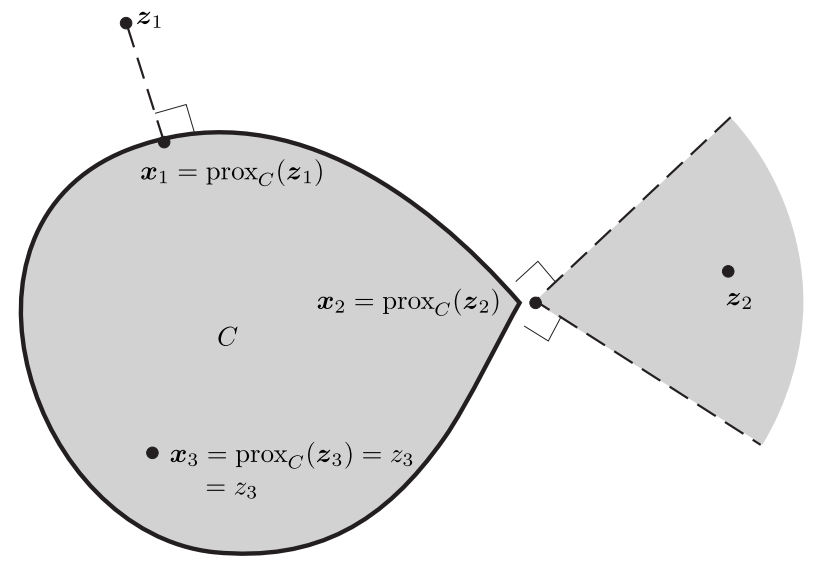
\includegraphics[width=.6\textwidth]{convex.PNG}\caption{}\label{fig:convex}
\end{figure}

This formulation can be used to define Signourini's contact law, which is defined as \eqref{eq:ncpcontact2}. The normal cone formulation, as illustrated in Figure~\ref{fig:convex}, of the contact is given by

\begin{align}
-h_{n,i} \in N_{C_{n,i}}(\lambda_{n,i}),\quad \text{with }C_{n,i} = (\Rbb^n)^+.\label{eq:hnormalcone}
\end{align}
The set $C_{n,i}$ is the set of admissible normal forces according to Signourini's law. See Figure~\ref{fig:signourinicontact} for an illustration of the set $C_{n,i}$ with $\lambda_{n,i}\in C_{n,i}$ and $h_{n,i} \in N_{C_{n,i}}(\lambda_{n,i})$. Now using the fact that
\begin{align}
\xb = \prox_C(\xb -r\yb), r > 0\ \iff\ -\yb\in N_C(\xb),
\end{align}
rewriting \eqref{eq:hnormalcone} to a proximal point formulation gives 

\begin{align}
\lambda_{n,i} = \prox_{C_{n,i}}(\lambda_{n,i} - rh_{n,i}),\quad \text{with }C_{n,i} = (\Rbb^n)^+\text{ and } r>0.
\end{align}

Similarly for the Poisson's impact law illustrated in Figure~\ref{fig:poissonimpact}, we find the proximal point formulation

\begin{align}
\Lambda_{n,i} = \prox_{C_{n,i}}(\Lambda_{n,i} - r\zeta^+_{n,i}),\quad \text{with }C_{n,i} = (\Rbb^n)^+\text{ and } r>0.
\end{align}

\subsection{Coulomb's friction law}
Now we define the normal cone formulation of Coulomb's friction law
\begin{align}
-\zetab_{t,i} \in N_{C_{t,i}}(\lambdab_{t,i})\quad \forall i\in\Ic_a,\quad \text{with }C_{t,i}(\lambda_{n,i}) = \{\lambdab_{t,i}\ |\ ||\lambdab_{t,i}|| \leq \mu\lambda_{n,i}\},
\end{align}
which is illustrated in Figure~\ref{fig:frictiondisk}.  

\begin{figure}[h]
\centering
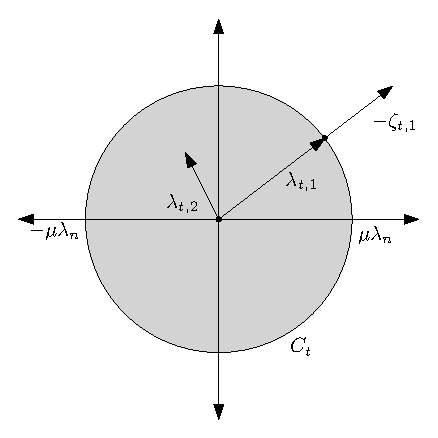
\includegraphics[width=.4\textwidth]{frictiondisk.eps}\caption{The friction disk with two seperate friction forces $\lambdab_{t,1}$ and $\lambdab_{t,2}$. $\lambdab_{t,1} = \mu\lambda_{n,1}$, resulting in a tangential velocity $\zetab_{t,i}>0$. $\lambdab_{t,2}<\mu\lambda_{n,2}$, leading to a tangential velocity $\zetab_{t,i}=0$.}\label{fig:frictiondisk}
\end{figure}

$C_t$ is the set of all admitted friction forces. The tangential velocity $\zetab_{t,i}$ is directed opposite to the friction force $\lambdab_{t,i}$ for isotropic friction. 

Now using the fact that
\begin{align}
\xb = \prox_C(\xb -r\yb), r > 0\ \iff\ -\yb\in N_C(\xb),
\end{align}
we can rewrite the normal cone to a proximal point formulation
\begin{align}
\lambdab_{t,i} = \prox_{C_{t,i}}(\lambdab_{t,i} - r\zetab_{t,i})\,\quad\text{with }C_{t,i}(\lambda_{n,i}) = \{\lambdab_{t,i}\ |\ ||\lambdab_{t,i}|| \leq \mu\lambda_{n,i}\}\text{ and }r>0.
\end{align}
Similarly, for the impact dynamics we can formulate
\begin{align}
\Lambdab_{t,i} = \prox_{C_{t,i}}(\Lambdab_{t,i} - r\zetab^+_{t,i})\,\quad \text{with }C_{t,i}(\lambda_{n,i}) = \{\Lambdab_{t,i}\ |\ ||\Lambdab_{t,i}|| \leq \mu\Lambda_{n,i}\}\text{ and }r>0.
\end{align}

\subsection{System dynamics with contact law and friction law}
The flow dynamics is then described by
\begin{align}
&\Mb(\qb)\dot{\xib} + \Hb(\qb,\xib) = \Sb(\qb)\ub + \sum_{i\in\Ic_c}\left(\wb_{n,i}(\qb)\lambda_{n,i} + \Wb_{t,i}(\qb)\lambdab_{t,i} \right), \label{eq:proxcontact1}\\
&\lambda_{n,i} = \prox_{C_{n,i}}(\lambda_{n,i} - rh_{n,i}),\label{eq:proxcontact2}\\
&\lambdab_{t,i} = \prox_{C_{t,i}}(\lambdab_{t,i} - r\zetab_{t,i}),\label{eq:proxcontact3}
\end{align}
with
\begin{align}
&C_{n,i} = (\Rbb^n)^+\text{ and } r>0,\\
&C_{t,i}(\lambda_{n,i}) = \{\lambdab_{t,i}\ |\ ||\lambdab_{t,i}|| \leq \mu\lambda_{n,i}\}\text{ and }r>0.
\end{align}
The impulsive dynamics that take place when a contact point opens or closes contact is described by
\begin{align}
&\Mb(\qb)(\xib^+ - \xib^-) = \sum_{i\in\Ic_c}\left( \wb_{n,i}(\qb)\Lambda_{n,i} + \Wb_{t,i}(\qb)\Lambdab_{t,i}\right), \label{eq:proximpact1}\\
&\Lambda_{n,i} = \prox_{C_{n,i}}(\Lambda_{n,i} - r\zeta^+_{n,i}),\label{eq:proximpact2}\\
&\Lambdab_{t,i} = \prox_{C_{t,i}}(\Lambdab_{t,i} - r\zetab^+_{t,i})\,\label{eq:proximpact3}
\end{align}
with
\begin{align}
&C_{n,i} = (\Rbb^n)^+\text{ and } r>0,\\
&C_{t,i}(\lambda_{n,i}) = \{\Lambdab_{t,i}\ |\ ||\Lambdab_{t,i}|| \leq \mu\Lambda_{n,i}\}\text{ and }r>0.
\end{align}
\section{Hybrid system formulation for mechanical system with unilateral constraints and spatial friction}
In this section the dynamics of the complementarity system defined in Section~\ref{sec:comp} is written to a hybrid formulation. 

\subsection{Hybrid system formulation}
\begin{align}
&\Mb(\qb)\ddot{\qb} + \Hb(\qb,\dot{\qb}) = \Sb(\qb)\ub + \sum_{i\in\Ic_c}\left(\wb_{n,i}(\qb)\lambda_{n,i} + \Wb_{t,i}(\qb)\lambdab_{t,i} \right), \label{eq:hybriddyn}
\end{align}
where every contact point is subjected to some set of constraints $c_i$, depending on the mode the contact point is in. The outline of the hybrid system is given below, in which the constraints, guard functions and jump maps will be derived in Section~\ref{app:constraints}, \ref{app:guards} and \ref{app:jumpmaps} respectively.

\textbf{Open:}\\
Set of constraints on the contact in flow are given by
\begin{align}
&c_{\text{open},i}:\nonumber\\
&\lambda_{n,i} = 0,\\
&\lambdab_{t,i} = 0,
\end{align}
and the jump sets are given by
\begin{align}
^{\text{slip}\leftarrow \text{open}}\mathcal{D} &= \{\qb,\ub\in\Rbb^n,\Rbb^m:\ ^{\text{closed}\leftarrow \text{open}}\gamma = 0,\ ^{\text{closed}\leftarrow \text{open}}\dot{\gamma}<0,\ ^{\text{slip,stick}}\Gamma < 0 \},\label{eq:D0to1}\\
^{\text{stick}\leftarrow \text{open}}\mathcal{D} &= \{\qb,\ub\in\Rbb^n,\Rbb^m:\ ^{\text{closed}\leftarrow \text{open}}\gamma = 0,\ ^{\text{closed}\leftarrow \text{open}}\dot{\gamma}<0,\ ^{\text{slip,stick}}\Gamma \geq 0 \},\label{eq:D0to2}
\end{align}
with 
\begin{align}
^{\text{closed}\leftarrow \text{open}}\gammab &= h_{n,i},\\
^{\text{slip,stick}}\Gamma &= \mu^2 \Lambda_{n,i}^2(\qb,\dot{\qb}^-) - \Lambdab_{t,i}(\qb,\dot{\qb}^-)\Lambdab_{t,i}^T(\qb,\dot{\qb}^-).
\end{align}
\textbf{Slip:}\\
Set of constraints on the contact in flow are given by
\begin{align}
&c_{\text{slip},i}:\nonumber\\
&\wb^T_{n,i}(\qb)\ddot{\qb} + \dot{\wb}^T_{n,i}(\qb)\dot{\qb} = 0,\\
&\lambdab_{t,i} = -\widehat{\zetab}^-_{t,i}\mu\lambda_{n,i},
\end{align}
where $\widehat{\zetab}^-_{t,i}$ is the vector length of $\zetab^-_{t,i}$ as defined in \eqref{eq:vectorlen} and the jump sets are given by
\begin{align}
^{\text{open}\leftarrow \text{slip}}\mathcal{D} &= \{\qb,\ub\in\Rbb^n,\Rbb^m:\ ^{\text{open}\leftarrow \text{closed}}\gamma = 0,\ ^{\text{open}\leftarrow \text{closed}}\dot{\gamma} < 0 \},\\
^{\text{stick}\leftarrow \text{slip}}\mathcal{D} &= \{\qb,\ub\in\Rbb^n,\Rbb^m:\ ^{\text{stick}\leftarrow \text{slip}}\gamma = 0,\ ^{\text{stick}\leftarrow \text{slip}}\dot{\gamma} < 0 \},
\end{align}
with
\begin{align}
^{\text{open}\leftarrow \text{closed}}\gamma &= \lambda_{n,i},\\
^{\text{stick}\leftarrow \text{slip}}\gamma &= \zetab^T_{t,i}\zetab_{t,i}.
\end{align}
\textbf{Stick:}\\
Set of constraints on the contact in flow are given by
\begin{align}
&c_{\text{stick},i}:\nonumber\\
&\wb^T_{n,i}(\qb)\ddot{\qb} + \dot{\wb}^T_{n,i}(\qb)\dot{\qb} = 0,\\
&\Wb^T_{t,i}(\qb)\ddot{\qb} + \dot{\Wb}^T_{t,i}(\qb)\dot{\qb} = 0,
\end{align}
and the jump sets are given by
\begin{align}
^{\text{open}\leftarrow \text{stick}}\mathcal{D} &= \{\qb,\ub\in\Rbb^n,\Rbb^m:\ ^{\text{open}\leftarrow \text{closed}}\gamma = 0,\ ^{\text{open}\leftarrow \text{closed}}\dot{\gamma} < 0 \},\\
^{\text{slip}\leftarrow \text{stick}}\mathcal{D} &= \{\qb,\ub\in\Rbb^n,\Rbb^m:\ ^{\text{slip}\leftarrow \text{stick}}\gamma = 0,\ ^{\text{slip}\leftarrow \text{stick}}\dot{\gamma} < 0 \},
\end{align}
with
\begin{align}
^{\text{open}\leftarrow \text{closed}}\gamma &= \lambda_{n,i},\\
^{\text{slip}\leftarrow \text{stick}}\gamma &= \mu^2\lambda_{n,i}^2 - \lambdab^T_{t,i}\lambdab_{t,i}.
\end{align}

The states that enter a jump set will be mapped to the corresponding flow set, and experience a state reinitialization according to the jump maps
\begin{align}
&\text{open}\leftarrow \ast:\nonumber\\
&(\dot{\qb}^+ - \dot{\qb}^-) = 0,\\
&\text{slip}\leftarrow\ast:\nonumber\\
&\Mb(\qb)(\dot{\qb}^+ - \dot{\qb}^-) = \wb_{n,i}(\qb)\Lambda_{n,i} + \Wb_{t,i}(\qb)\Lambdab_{t,i},\\
&\zeta_{n,i}^+=0,\\
&\Lambdab_{t,i} = -\widehat{\zetab}^-_{t,i}\mu\Lambda_{n,i},\\
&\text{stick}\leftarrow \ast:\nonumber\\
&\Mb(\qb)(\dot{\qb}^+ - \dot{\qb}^-) = \wb_{n,i}(\qb)\Lambda_{n,i} + \Wb_{t,i}(\qb)\Lambdab_{t,i},\\
&\zeta_{n,i}^+=0,\\
&\zeta_{t,i}^+= 0,
\end{align}
where $\ast$ represents an arbitrary mode. For example, a transition from any ante-event mode to an open post-event mode will use the jump map $\text{open}\leftarrow \ast$.
%\begin{figure}[H]
%\centering
%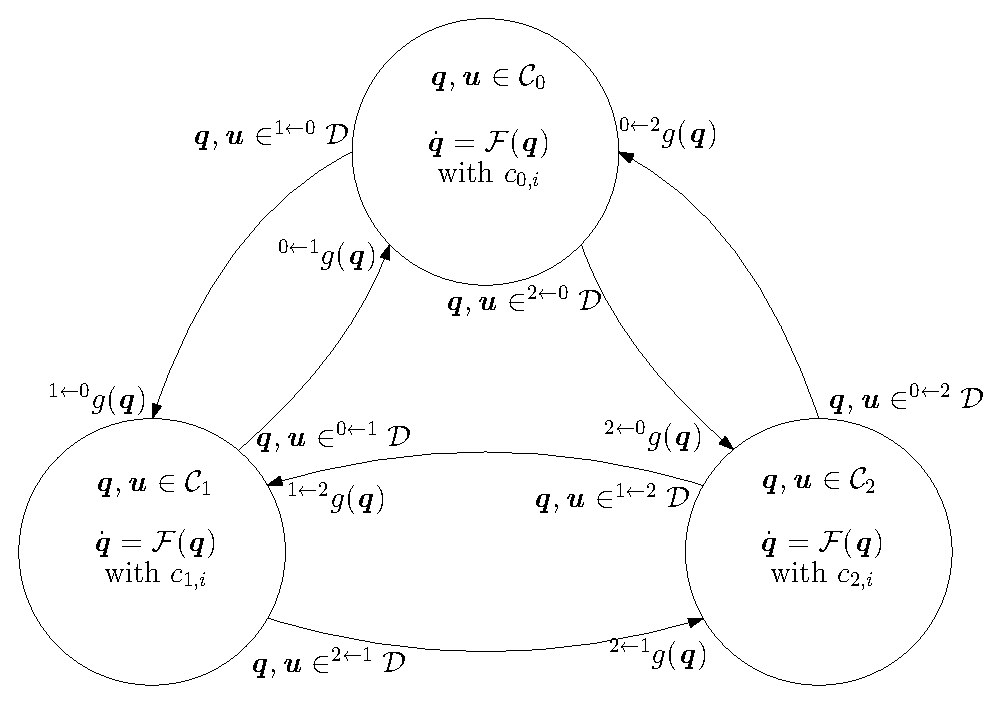
\includegraphics[width=.8\textwidth]{nodehybrid.eps}\caption{The hybrid system representation of one contact point of a system experiencing impact and spatial friction.}\label{fig:nodehybrid}
%\end{figure}

\textbf{THE FOLLOWING SUBSECTIONS STILL HAVE TO BE WRITTEN}
\subsection{Flow set constraint derivation}\label{app:constraints}


\subsection{Guard-function derivation}\label{app:guards}
\textbf{Open to stick/slip}\\
When a contact point is "open", it can trigger a guard function $\gamma$ to go from open to closed.

\textbf{DEFINITION OF $\gamma$}

The plane that spans $\gamma = 0$ is divided in two regions: a region where the post-impact state is in slip and a region where the post-impact state is in stick. This region is defined by $\Gamma$, where $\Gamma<0$ in the region where the contact point goes to slip and $\Gamma > 0$ in the region where the contact point goes to stick. When $\Gamma = 0$ the system is right at the border between a slip post-impact state and a stick post-impact state. This is illustrated in Figure~\ref{fig:guardopcl}. 

\begin{figure}[H]
	\centering
	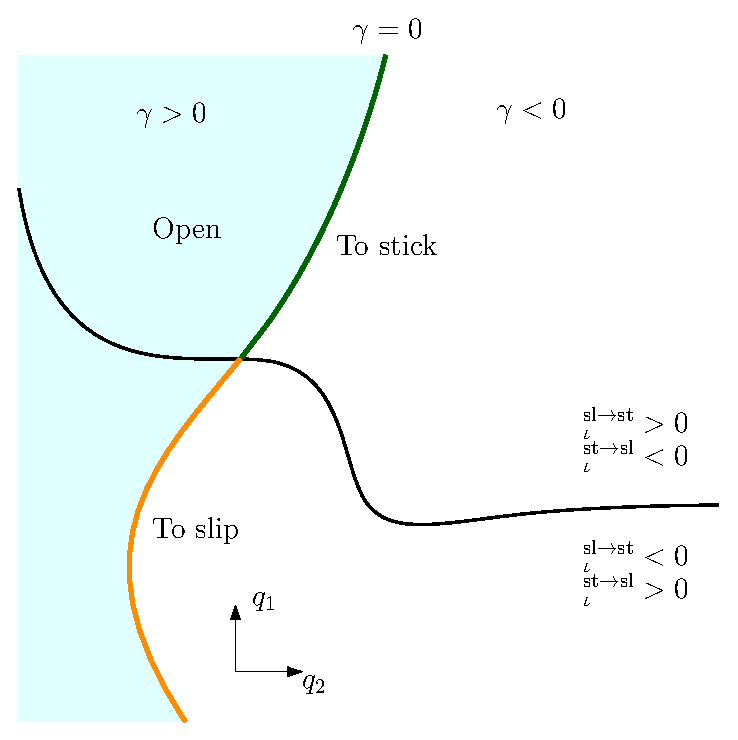
\includegraphics[width=.7\textwidth]{guardopcl.eps}\caption{The functions $\gammab(\qb,\dot{\qb})$ and $\Gammab(\qb,\dot{\qb})$ illustrated in the state space of $\qb\in\mathbb{R}^{2}$. The light blue area is the state space where the contact is open, and goes the closed when it triggers $\gamma = 0$. If it triggers $\gamma = 0$ in the area where $\Gamma<0$ (orange), then the contact will go to slip. If it triggers $\gamma=0$ in the area where $\Gamma\geq 0$ (green), then the contact will go to stick.}\label{fig:guardopcl}
\end{figure}

For slip, we know that $\mu\Lambda_{n,i} - ||\Lambdab_{t,i}|| = 0$ and for stick, we know that  $\mu\Lambda_{n,i} - ||\Lambdab_{t,i}|| \geq 0$. From this we can derive the guard function
\begin{align}
\Gamma = \mu^2 \Lambda_{n,i}^2(\qb,\dot{\qb}^-) - \Lambdab_{t,i}(\qb,\dot{\qb}^-)\Lambdab_{t,i}^T(\qb,\dot{\qb}^-). \label{eq:slipset}
\end{align}
This guard function $\Gamma$ satisfies the requirements that $\Gamma<0$ in the region where the contact point goes to slip, $\Gamma > 0$ in the region where the contact point goes to stick and $\Gamma = 0$ at the border. Even though it is not physically realistic that $\Gamma < 0$, it can still be used as a guard-function.
We now find expressions for $\Lambda_{n,i}$ and $\Lambdab_{t,i}$ by looking at the jump map to stick, given in \eqref{eq:appjump5} to \eqref{eq:appjump7}.

We can rewrite \eqref{eq:appjump5} to
\begin{align}
\dot{\qb}^+ = \Mb^{-1}\wb_{n,i}\Lambda_{n,i} + \Mb^{-1}\Wb_{t,i}\Lambdab_{t,i} + \dot{\qb}^-,
\end{align}
which after substituting into \eqref{eq:appjump6} and \eqref{eq:appjump7} lead to

\begin{align}
\wb_{n,i}^T\Mb^{-1}\wb_{n,i}\Lambda_{n,i} + \wb_{n,i}^T\Mb^{-1}\Wb_{t,i}\Lambdab_{t,i} + \zeta_{n,i}^- = 0\\
\Wb_{t,i}^T\Mb^{-1}\wb_{n,i}\Lambda_{n,i} + \Wb_{t,i}^T\Mb^{-1}\Wb_{t,i}\Lambdab_{t,i} + \zetab_{t,i}^- = 0,
\end{align}
respectively, with $\zeta_{n,i}^- = \wb_{n,i}^T\dot{\qb}^-$ and $\zetab_{t,i}^- = \Wb_{t,i}^T\dot{\qb}^-$. This is now rewritten to

\begin{align}
\begin{bmatrix}
\wb_{n,i}^T\Mb^{-1}\wb_{n,i} & \wb_{n,i}^T\Mb^{-1}\Wb_{t,i} \\
\Wb_{t,i}^T\Mb^{-1}\wb_{n,i} & \Wb_{t,i}^T\Mb^{-1}\Wb_{t,i}
\end{bmatrix}
\begin{bmatrix}
\Lambda_{n,i}\\
\Lambdab_{t,i}
\end{bmatrix} + \begin{bmatrix}
\zeta_{n,i}^-\\
\zetab_{t,i}^-
\end{bmatrix}
= 0,
\end{align}
which is in turn rewritten to
\begin{align}
\begin{bmatrix}
\Lambda_{n,i}\\
\Lambdab_{t,i}
\end{bmatrix} = - \Db^{-1}\begin{bmatrix}
\zeta_{n,i}^-\\
\zetab_{t,i}^-
\end{bmatrix},\quad \text{with } \Db = \begin{bmatrix}
\wb_{n,i}^T\Mb^{-1}\wb_{n,i} & \wb_{n,i}^T\Mb^{-1}\Wb_{t,i} \\
\Wb_{t,i}^T\Mb^{-1}\wb_{n,i} & \Wb_{t,i}^T\Mb^{-1}\Wb_{t,i}
\end{bmatrix}.
\end{align}

The matrix $\Db$ is often called a Delassus-matrix. We now have expressions for $\Lambda_{n,i}$ and $\Lambdab_{t,i}$ which are continuous and differentiable in $(\qb,\dot{\qb})$. It is straightforward that $\Gamma(\qb,\dot{\qb})$ is continuous and differentiable as well.

\textbf{Stick to slip and slip to stick}\\

\textbf{Stick/slip to open}\\



\subsection{Jump map derivation}\label{app:jumpmaps}
The impact dynamics related to the jump sets are given by
\begin{align}
&0\leftarrow \ast:\nonumber\\
&(\dot{\qb}^+ - \dot{\qb}^-) = 0,\label{eq:appjump1}\\
&1\leftarrow\ast:\nonumber\\
&\Mb(\qb)(\dot{\qb}^+ - \dot{\qb}^-) = \wb_{n,i}(\qb)\Lambda_{n,i} + \Wb_{t,i}(\qb)\Lambdab_{t,i},\label{eq:appjump2}\\
&\zeta_{n,i}^+=0,\label{eq:appjump3}\\
&\Lambdab_{t,i} = -\widehat{\zetab}^-_{t,i}\mu\Lambda_{n,i},\label{eq:appjump4}\\
&2\leftarrow \ast:\nonumber\\
&\Mb(\qb)(\dot{\qb}^+ - \dot{\qb}^-) = \wb_{n,i}(\qb)\Lambda_{n,i} + \Wb_{t,i}(\qb)\Lambdab_{t,i},\label{eq:appjump5}\\
&\zeta_{n,i}^+=0,\label{eq:appjump6}\\
&\zeta_{t,i}^+= 0,\label{eq:appjump7}
\end{align}
with $0\leftarrow\ast$,$1\leftarrow\ast$ and $2\leftarrow\ast$ representing the impact dynamics to open contact, slip and stick respectively. 

When we go from any mode to open, there is no jump in the velocity and the reaction impulses are 0. Therefore $0\leftarrow \ast$ is correct.

When we go from open to slip, there will be a jump in velocity, and $||\Lambdab_{t,i}|| = \mu\Lambda_{n,i}$. The reaction impulses will be larger than zero. When we go from stick to slip, there will be no jump in velocity. In stick, $\zetab_{t,i} =0$, so $\epsilon(\zetab^-_{t,i}) = 0$. Also we know $\wb_{n,i}^T\dot{\qb}^- = \wb_{n,i}^T\dot{\qb}^+ = 0 $. This leads to $\dot{\qb}^- = \dot{\qb}^+$, meaning there is no jump in velocity and no impulsive reaction force. Therefore $1\leftarrow \ast$ is correct.

When we go from open to stick, there will be a jump in velocity and impulsive reaction forces.
\textbf{SHOW THAT JUMP MAPS ARE CORRECT}

\cleartooddpage
\chapter{Trajectory Tracking Control for Hybrid Systems with State-Triggered Jumps}
\cite{Rijnen2017}
\section{Error notation for perturbed jump times}
\section{Linearization for Trajectories with Separate Guard-Activation}

\end{document}